\makeatletter

\pgfplotsset{
    /tikz/max node/.style={
        anchor=south
    },
    /tikz/min node/.style={
        anchor=north
    },
    mark min/.style={
        point meta rel=per plot,
        visualization depends on={x \as \xvalue},
        scatter/@pre marker code/.code={%
            \ifx\pgfplotspointmeta\pgfplots@metamin
                \def\markopts{}%
                \coordinate (min);
                \node [min node] (minlabel) {
                    \pgfmathprintnumber[fixed]{\xvalue},%
                    \pgfmathprintnumber[fixed,precision=5]{\pgfplotspointmeta}
                };
            \else
                \def\markopts{mark=none}
            \fi
            \expandafter\scope\expandafter[\markopts,every node near coord/.style=green]
        },%
        scatter/@post marker code/.code={%
            \endscope
        },
        scatter,
    },
    mark max/.style={
        point meta rel=per plot,
        visualization depends on={x \as \xvalue},
        scatter/@pre marker code/.code={%
        \ifx\pgfplotspointmeta\pgfplots@metamax
            \def\markopts{}%
            \coordinate (max);
            \node [max node] (maxlabel){
                \pgfmathprintnumber[fixed]{\xvalue},%
                \pgfmathprintnumber[fixed,precision=5]{\pgfplotspointmeta}
            };
        \else
            \def\markopts{mark=none}
        \fi
            \expandafter\scope\expandafter[\markopts]
        },%
        scatter/@post marker code/.code={%
            \endscope
        },
        scatter
    }
}
\makeatother


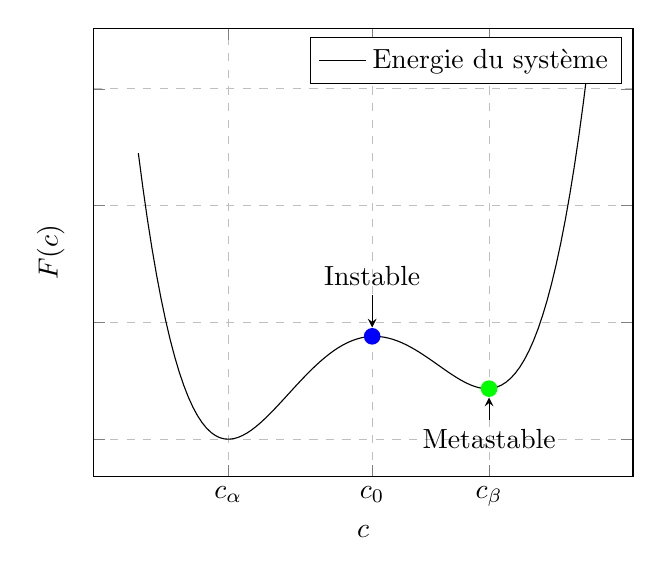
\begin{tikzpicture}
\begin{axis}[
%axis lines = left,
xlabel = \(c\),
ylabel = {\(F(c)\)},
xmajorgrids=true,
ymajorgrids=true,
scaled ticks=false,
xticklabel=\empty,
yticklabel=\empty,
xtick={0.4,0.56, 0.69},
% extra x tick style={grid=none},
xticklabels={%
{$c_\alpha$},
{$c_0$},
{$c_\beta$}
},
grid style=dashed,
] % end axis options

\def\Vb{0.05}
\addplot[
domain=0.3:0.8,
samples=100,
color=black
]% end plot options
{15*((x-0.4)^2 * (0.7-x)^2) + (x-0.4)^2*\Vb}; % end plot func
\addlegendentry{Energie du système}



% \addplot[
% domain=0.5:0.7,
% samples=100,
% color=red, mark min, every node near coord/.style=
% ]% end plot options
% {15*((x-0.4)^2 * (0.7-x)^2) + (x-0.4)^2*\Vb}; % end plot func
% \addplot[
% domain=0.4:1.1,
% samples=100,
% color=red, mark max, every node near coord/.style=
% ]% end plot options
% {x^2 * (1-x)^2 + x*\Vb}; % end plot func

\node (label_unstable) at (axis cs:0.56,0.014) {Instable};
\node (label_metastable) at (axis cs:0.69,0.0) {Metastable};

\node[circle,fill, blue, minimum size=6pt, inner sep=0] (unstable) at (axis cs: 0.56,0.00881) {};
\node[circle,fill, green, minimum size=6pt, inner sep=0] (metastable) at (axis cs: 0.69,0.00433) {};
\draw[-stealth] (label_metastable) to [out=90,in=-90] (metastable.south);
\draw[-stealth] (label_unstable) to [out=-90,in=90] (unstable.north);
\end{axis}

% \coordinate (a) at (current bounding box.south);
% \coordinate (b) at (current bounding box.north);
% \pgfresetboundingbox
% \useasboundingbox  (a) rectangle (b);

\end{tikzpicture}

